\documentclass{article}

\usepackage[dutch]{babel}
\usepackage[version=3]{mhchem}
\usepackage{hyperref}
\usepackage{pdfpages}
\usepackage{graphicx}
 
\usepackage{marvosym}
\usepackage{url} 

\begin{document}

\title{Documentatie Pinautomaat}
\author{Bytegroep 10}

\maketitle

\begin{abstract}

Wij moesten...

\end{abstract}

\newpage

\section{Beheren}

\subsection{Versiebeheer}

Voor dit onderdeel moesten wij kunnen werken met Git en Version control.
Hier is veel onderzoek over gedaan zodat het goed toegepast kan worden dit project.
In figuur \ref{fig: git model} is het model wat wij gebruiken op onze Git pagina, \href{https://github.com/Gewad/Project4Bankalicious}{Project4Bankalicious}.
Ieder groepslid werkt op zijn individuele branch, en als je klaar bent met jouw onderdeel, dan wordt hij in test gemerged.
Als er geen problemen lijken te zijn op de test beslissen wij in een groep of wij test naar de master kunnen schrijven.
Alle documentatie is terug te vinden op Github.

\begin{figure}[!h]
        \centering
        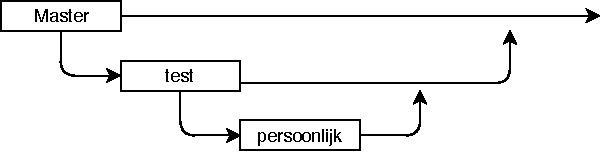
\includegraphics[height=0.7in]{git.pdf}
        \caption{git model}
        \label{fig: git model}
\end{figure}

\section{Analyse \& advies}

\subsection{Dispenser}

Wij hebben onderzoek gedaan naar twee manieren van het uitgeven van biljetten.
Wij hebben vooral onderzoek gedaan bij de tweede jaars.
Optie \'e\'en is om een zuigpomp te gebruiken en de biljetten naar boven te zuigen.
De tweede jaars raden dit af, omdat zij hier zelf geen goede ervaring mee hadden.

Manier twee is om de biljetten uit te werpen met een elektromotor.
De tweede jaars hadden hier goede ervaring mee, dit ding namelijk minder vaak fout bij het uitwerpen.
De elektromotor zal de kaarten uit de dispenser rollen.

Voor het uitgeven van biljetten is het effici\"enter om een elektromotor te gebruiken.
Hier is er meer kans dat het juiste aantal biljetten uit de automaat komen.

\newpage

\subsection{Veiligheid}

\paragraph{Netwerk encryption}

Er is veel onderzoek gedaan naar de beveiliging van het dataverkeer.
Voor netwerken beveiliging heb je een encryptie nodig over het netwerk.
Wij raden aan om hiervoor een bestaand protocol toe te passen.
SSL wordt professioneel toegepast bij bedrijven.
Het kan gewoon gebruikt worden als hij goed toegepast wordt met de meest recente versie.

\paragraph{lokale encryption}

Voor lokale encryption zou je de hele database kunnen encrypten, en decrypten wanneer je data nodig hebt.
Dit kost echter een hoop rekenkracht, en je gegevens zullen op een paar plaatsen onversluiteld zijn.

Een oplossing hiervoor is om gevoelige gegevens te hashen, en vervolgens in de database op te slaan.
Als je bijvoorbeeld wilt controleren of een pincode klopt, zal deze eerst gehasht worden en vervolgens vergeleken met wat er in de database staat.
Een veelgebruikt hashing algoritme voor java en c++, de talen waar wij in programmeren, is bijvoorbeeld md5.
Het is beter om een hashing algoritme te gebruiken wat iets zwaarder is dan md5, omdat je een hash makkelijk terug kunt rekenen.
Een beter veelgebruikt algoritme is bijvoorbeeld SHA1.
Deze adviseren wij te gebruiken.

\hfill

\centerline{\ce{pincode ->[hash] hashed} \ce{pincode} \ce{->[vergelijk] Database met hashes}}

\paragraph{Afgesloten hardware}

Het is heel cruciaal voor de automaat dat buitenstaanders geen toegang hebben tot de logica van de machine en de biljetten.
Om dit te voorkomen is het het handigst om de hardware aan de binnenkant van de automaat te houden.
Wij raden aan om een kast om de functionele onderdelen heel te bouwen, zodat deze niet meer toegankelijk zijn.

\subsection{Biljetten}

Wij hebben eerst aan de tweede jaars gevraagd wat voor soort materiaal wij het best konden gebruiken voor de biljetten.
Zij kwamen met twee opties.
\begin{itemize}
\item Je kan zelf biljetten maken, om ze zo op je model af te stellen.
\item Je kan speelkaarten gebruiken, omdat deze gemaakt zijn om met een dispenser uit te werpen.
\end{itemize}

Wij raden aan om speelkaarten te gebruiken.
Het zou extra tijd kosten om zelf kaarten te maken.
Wij kunnen direct aan te slag met de dispenser als wij speelkaarten gebruiken, sinds wij deze al hebben.

TODO Paul help deze redenen zijn kut.

\newpage

\subsection{Sorteren van biljetten}

Wat bedoel je met sorteren?

\subsection{Materiaal}

Hout, want snijder.

\subsection{Communicatie}

TODO Netwerk model

\section{Ontwerp \& realisatie}

\subsection{Bouwtekening ATM}

Kijk wij kunnen tekenen!

\subsection{Testen}

Tijdens het testen...
Dit dat blijkt kut...
Dit dat zo gefixed...

\end{document}
